\documentclass[11pt, a4paper]{article}

\usepackage[utf8]{inputenc}
\usepackage{graphicx}
\graphicspath{ {images/} }
\usepackage{mathtools}
\usepackage{amssymb}
\usepackage{amsmath}
\usepackage[ngerman,english]{babel}
\usepackage{cite}
\usepackage{bibgerm}
\usepackage[top=0.0cm,bottom=1.5cm,left=3.5cm,right=3.5cm,headsep=1.5cm,includeheadfoot]{geometry}
\usepackage{tabularx}
\usepackage{eurosym}
\usepackage{enumitem}
\usepackage{multicol}
\usepackage{tikz}
\usepackage{tkz-euclide}
\usepackage{pgfplots}
\usepackage{pdflscape}
\usepackage{wrapfig}
\usepackage{acronym}
\usepackage{blindtext}
\usepackage{ifthen}
\usepackage{setspace}
\usepackage{cancel}
\usepackage{color}
\usepackage{listings}
\usepackage{comment}
\usepackage{xcolor}
\usepackage{colortbl}

\usetikzlibrary{graphs}
\usetikzlibrary{positioning}

\onehalfspacing
\setlength\parindent{0pt}

\everymath{\displaystyle}

\allowdisplaybreaks

\definecolor{AIblue}{rgb}{0,0.57,0.87}
\definecolor{RUBblue}{rgb}{0,0.21,0.38}


\pagenumbering{gobble}

\title{Personal Reflection on the Study Project\\\textbf{Deep Convolutional Networks}}
\author{B. Sc. Christian Andreas Mielers (108 011 204 956)\\ B. Sc. Phil Yannick Schrör (108 011 214 024)}
\date{\today}

\begin{document}
\maketitle

Since we already worked together on many projects during the last 3 years, we have a lot of routine regarding our common work. Therefore we could start the project immediately after meeting our project supervisor Dr. Rolf P. Würtz for the first time.  Since the overall target of the project was to examine deep convolutional networks in general, we did not define milestones at the beginning of the project, but fixed and refined the targets of the study project step by step during the numerous discussions with our supervisor according to the results, which we achieved by and by during the semester.

Fortunately, we could realize almost all targets, which we agreed on. Solely one optional target (using a discretized approximation of the tangens hyperbolicus as activation function, cf. figure \ref{fig:discretized_tanh}) could not be realized without disproportional effort for technical reasons.

\begin{figure}[h!!!]
	\centering
	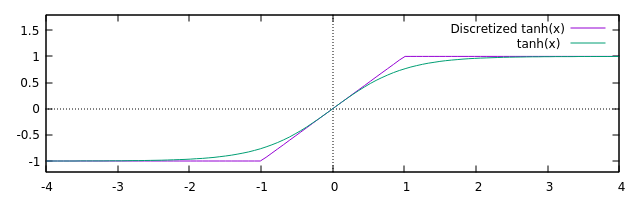
\includegraphics[width=1\textwidth]{discretized_tanh.png}
	\caption{Linear approximation of the tangens hyperbolicus}
	\label{fig:discretized_tanh}
\end{figure}

The major part of the time was spent on training convolutional neural networks on training data and subsequently testing them on previously unseen test datasets to evaluate the quality of the trained classifiers. In order to estimate the generalization properties of the trained filters, we visualized them graphically. Additionally we visualized the recognition rates on the test data after each training epoch by plotting them as function graph. With the help of these illustrations, it is easy to quickly extract the most important findings of our study project.

For all relevant information you are invited to study our main report.

\end{document}